\chapter{Design and Architecture}

The design of software application needs a well defined problem, when a new improved design of a user interface is needed. Main focus lays in easy navigation, responsive interface and intuitive access to the most needed parts of the system. Architecture describes ways of structuring software logic and communication.

\section{Flux and MVC}\label{sec:fluxmvc}
\subsection{What is MVC and Flux}
Two main software design patterns that were considered for this solution were Flux and MVC, React.js was set to be the main tool for using it as a view - (the part of the application that shows current data state), while researching React.js the preffered way to write the app for many programmers seemed to be Flux, although there was no clear advandage of Flux over MVC. MVC stands for Model View Controller, the first part, the model represents the logic, and data that is being displayed, the view is the part that displays the information the current data, and controller accepts the user input and sends it either to model or view, these are the main parts of the application that communicate with eachother. One can be very creative while implementing MVC, there exists many implementations of MVC, in general the flow inside MVC is not well defined, and when unexperienced programmer tries it, it can become very difficult to manage all the different parts, and it gets especcialy complicated when having a lot of different components that communicate with eachother. Even though Autograder is not as huge and complicated as some sites its still not a small application, there are many elements that depend on data from different places. One example would be the main part of the Autograder which is the lab overview where teachers can have an easy access to all the assignments and see individual results. 

\begin{figure}[h]
  {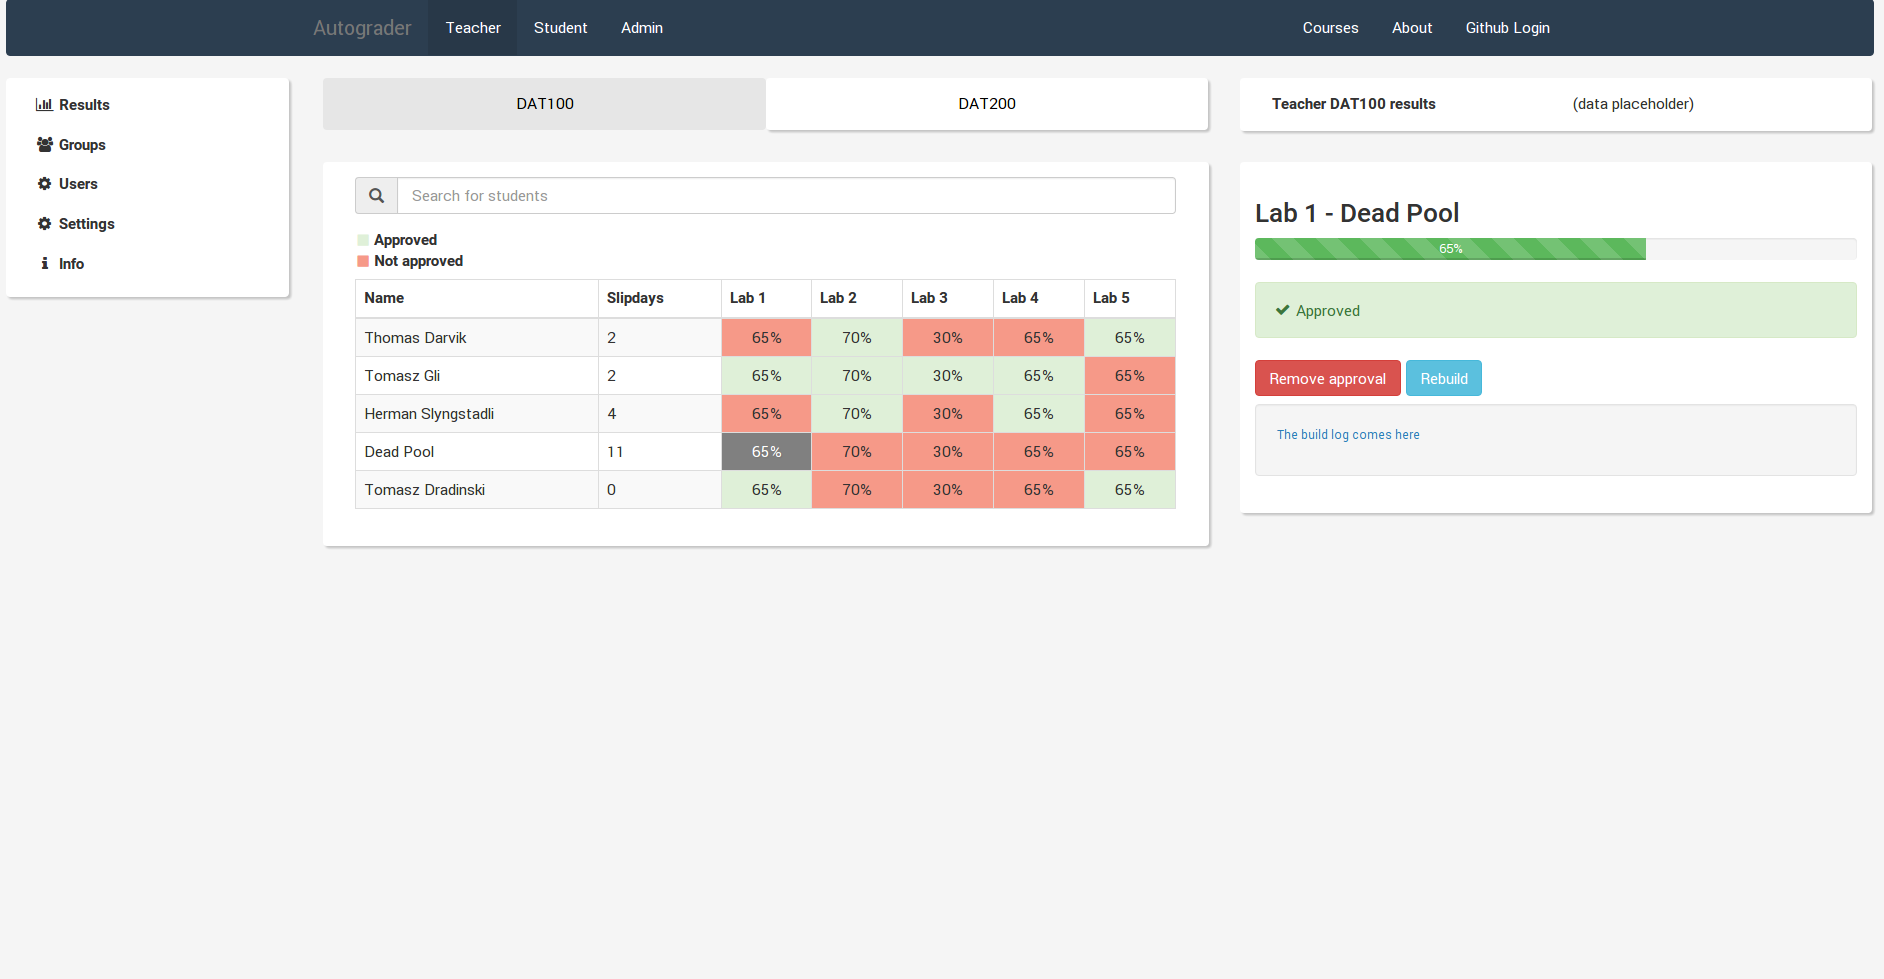
\includegraphics[width=1\linewidth]{laboverviewteacher}}
  \caption{The view that teacher sees when looking at all the labs in a given course}
  \label{fig:laboverwievteacher}
\end{figure}

The center section is a table of all the lab results for every student, to the right there is a expanded view of a selected lab (marked with gray).
Simple flowchart represented with MVC style design:

Other components;

\begin{tikzpicture}[scale=2]
  %nodes
  \node [block] (v1) at (0,0) {View LAB LIST};
  \node [block] (v2) at (2,1) {Controller LAB STATUS};
  \node [block] (v3) at (4,0) {Model LABS};
  \node [block] (v4) at (0,-1) {View LAB DETAILS};

  \draw [->] (v1) |- node [midway, above] {Choose lab} (v2);
  \draw [->] (v2) |- node [midway, below] {Update} (v1);
  \draw [->] (v2) -| node [midway, above] {Update} (v3);
  \draw [->] (v3) -| node {Notify} (2.3,0.57);
\end{tikzpicture}
  
\subsection{Why Flux}

\section{Design}

\subsection{User Interface Design}
The focus of new design lays in improving the user experience. Users of previous system, have shown dislike towards the UI design choices. The system is designed is such a way so that both students and teachers have intuitive access to the parts of the system that they use most frequently. There exists student section, teacher section, and also admin section, these major sections are designed so that it is obvious what parts of the system you have access to from the current section you are in. having Autograder in teacher mode, one can easily create a new course and rename it, GitHub integration \ref{gihubintegration} takes care of creating and managing the repositories needed in that course, initial setup of a course is done through a course settings page. The management of students that have joined the course, involves actions like organizing groups, expelling students and approving new students who joined the course, these can be done in the groups page and users page through easily accessible navigation. Most used functionality, by both teachers and teaching assistants is course lab overview. This results page lets a teacher quickly skim through all the students and look if anyone hasn't delivered their assignment yet, or see the score of each assignment, from there, it is also possible to approve or reject any given lab assignment. Another function is to be able to easily control group assignments, and assign students to specific groups. In the groups page, there exists a user friendly interface for creating new groups and adding available students to any given group, users can be notified about which group they have been assigned to, similarly, students can easily create groups that need to be approved by the teachers.
\\Students will utilize Autograder mainly for checking if their assignment has been approved. The default page for student section is lab overview, in there one can see the current assignment and its progress, it is also worth mentioning that usually one student wont be using Autograder in more than one course, but the system is designed for easy switch between different courses by using tabs to switch current page data with the relevant course information. There is no distinguished mode for teaching assistant, these are often students that are also registered as teachers in different course, this is where Autograder main sections come in handy, while working as a TA, user can switch to teacher mode and has access to the teachers functionality in the courses he teaches, similarly switching to student mode gives quick access to relevant functions in that mode.
\\As for admins of the system, there will usually be a handful of users with admin privileges, admins control access to the major sections of Autograder, when a user registers admins can assign teacher permissions for that user to be able to create new organizations and courses, and of course admins can upgrade other users to admins. Besides that there is a settings panel for admins that enables setting up initial setting for Autograder server, like hostname, passwords etc.
\subsection{Wireframes}
Creating wireframes is a crucial part of user interface design. The point of wireframes is to have something that is easier to change than the code to be developed. Before coming to the programming phase, one can iterate over a lot more design propositions, and is able to change things up easily during this initial or planning phase. Wireframes are foundation of the application being developed, they are not supposed to show the creative design, but rather reflect on the technological and use-related aspects of the application. Before the development of new user story takes action, sketches and drawings of user interface are being produced. This is done to eliminate flaws in the interface design before they are implemented, a couple of iterations of drawing are done and evaluated from the users perspective. When this initial phase is done, more sophisticated drawings or wireframes are being created. These more detailed drawings with descriptions of areas of the interface, describe what certain elements of this user interface do. Serving as a blue print for further developing of the interface.
\begin{figure}[h]
  {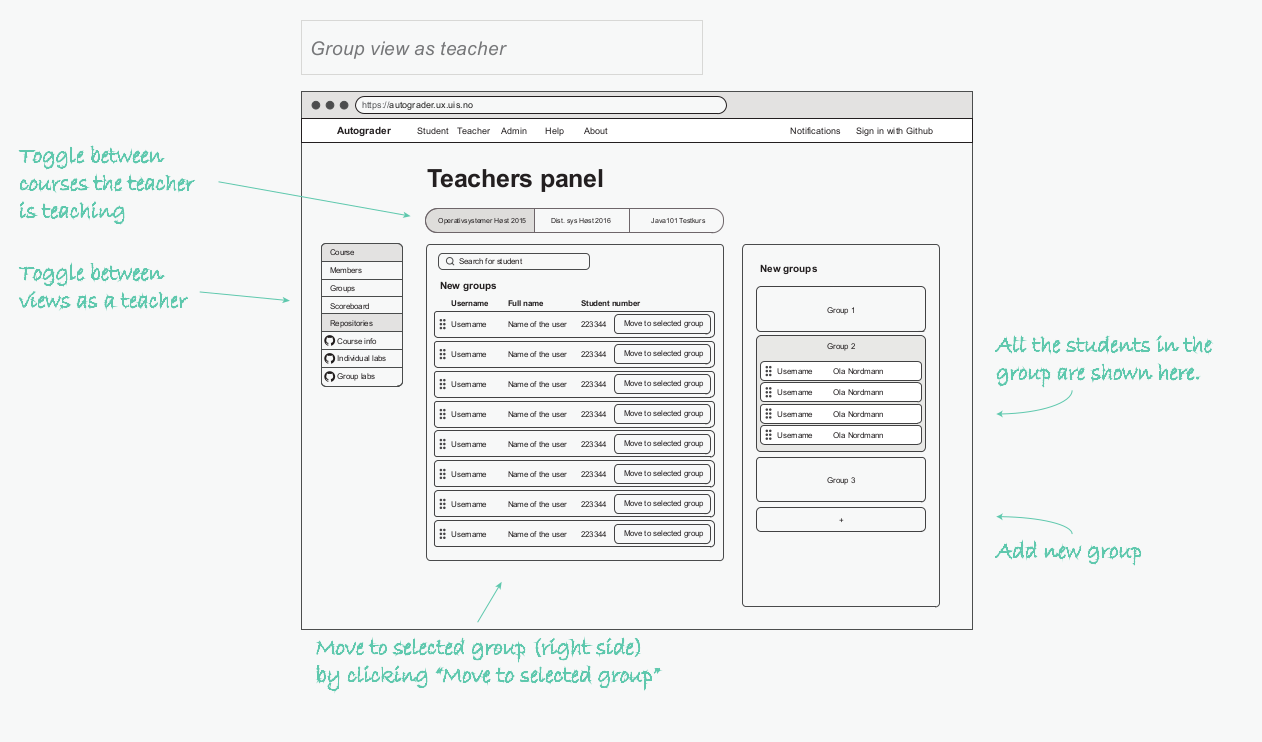
\includegraphics[width=1\linewidth]{groupmanagement}}
  \caption{Wireframes for Group management page}
  \label{fig:groupmanagement}
\end{figure}
\\Wireframes figure above was created as a result of a user story, next step is to create reflection of that Wireframes in code, 

\subsection{Planning of software solutions}
To achieve the goal of better, quicker and more responsive interface, the front-end application is written in JavaScript. By using new emerging open source technologies and libraries like React.js, it enabled quick and easy way to create a responsive user interface. In Model View Controller (more about it in section \ref{sec:fluxmvc}) React would stand for View, that is what user sees, and interacts with. What is missing is something to control the user interface and the data structures that it displays. This is achieved by structuring the application with one of many popular software architectures that are practiced nowadays. Slightly altered way of doing things than previous MVC implementations was introduced with Flux architecture. The way to write code with flux  pattern is to isolate every UI component and send every piece of data that user interacts with through a central hub that will dispatch it further, and other UI components can be set up to listen to those specific changes they are interested in, by forcing each UI action to go through whole system hierarchy instead of talking directly to another component we simplify debugging and most importantly make the logic much easier to understand, more about Flux in section \ref{sec:iflux}.
\\How the client communicates with the server is not relevant for the architecture and React.js. The communication implemented on this solution is called WebSocket protocol, in short this protocol establishes a constant connection with the server which is used to transfer data both ways in real time, updates can be send to the client from the server, there is no need for client to poll for any data. The connection is established after the initial GET request from the browser, client then asks for an "upgrade" to WebSocket protocol. The way client asks for data, is with a request string that represents the data payload that it is expecting to receive, the server associates every request with piece of data, client can also send additional payload such as username, limit for the size of the data e.g size of array list for pagination. More on WebSocket in section \ref{sec:websocket}.

\subsection{User stories}
User stories are a way to describe what application does, and what it is supposed to do in easy to read short descriptions. The focus here is to give a good fundament of what the applications is being developed for. Since there is a lot of functionality to be implemented, with the help of user stories is is possible to concentrate on one functionality described by that user story at a time. One example of a user story would be \emph{"As a teacher I want to be able to easily create groups for assignments, so that i don't have to approve student created groups."} fig: \ref{fig:groupmanagement}, \worry{choose better user story maybe?} this describes vaguely what a certain user would like to do with the application, but also can be created as a starting point for improvement to existing solution. It is also possible, by looking at this user story, to create a set of tasks that will guide through the steps of implementation. If there are parts of the system that need to be thought out again, or new solutions are needed to be in place before this functionality can be implemented, it is considered a part of the user story task. \worry{ With each new user story, the complexity of the application grows, and user interface should be theoretically improving on each cycle due to the way in which new functionality is implemented, since the flow of the application is being thought out and some initial design flaws might be discovered, things need to be either redesigned or a new solution found before this new functionality can be implemented. }\todo{More}

\section{Web app}
Architecture of the Autograder system describes the high level structures developed while working on the application. Choice of software architecture, software models on both front and back-end are crucial aspects of creating good application.
\subsection{Software architecture}
Autograder is an application for teachers and students, the new version is going to be running on local university network and is going to be accessible from anywhere on the internet, that means there is no restrictions as to what network you are trying to access it from. Primary use for teachers is creating courses in the Autograder system that are associated with the courses at the university, each course has a GitHub repository associated with it, and configured to the needs of that course. This means that an implementation of GitHub integration needs to be created, this is mainly the focus of back-end part of the software, still the front-end, or web client, needs to be designed in such a way to enable the use such integration. The client is not supposed to serve as an alternative view of GitHub repositories, GitHub is mainly used as a place to easily store source code, and its authentication system. The client needs to be able to display courses that a student is enrolled into, assignments that the teacher has published to that course, that also involves group assignments.
\\Although the data is stored in the database, manipulation of that data is done on the client side, and then sent further to the back-end for interpretation and updating the storage. Similarly it is also possible to update the client from the back-end, either directly or through the actions of another client. The user interface updates in real time, as an example, lets take a teacher that is assigning students to group assignments, teacher is using an interactive interface to manipulate the users into selected groups, the student is simultaneously notified in real time when he gets assigned to a new group without the need of refreshing the page \worry{better example here}. Teachers can be notified when a new student has enrolled to course, or one of the students has exceeded his slip-days for an assignment. Real time updates are possible due to the connection protocol used in the application. When a client connects to the Autograder server, client application requests for a protocol upgrade, from then on all data transfer is done through \emph{websocket protocol}\cite{websocket}. This enables the server to push its updates to all clients, without being explicitly asked about it by them.
\\The reasoning behind real-time update system was that notifications and responsiveness of user interface was one of the primary reasons for developing this application. Although one could argue that order methods of updating the UI and notifications would be sufficient, like polling or long-polling, that is frequent client requests for update from the server, websocket protocol has no obvious disadvantages to the presented solution, and at the same time opens possibilities for further upgrades of the system, like chat functionality, which could be utilized for questions related to assignments.
\subsection{Front-end}
\todo{single threaded approach}
\subsection{Angular}
\todo{discuss other methods than react, needs more research}
\subsection{React}
\todo{Would we use react for this purpose again?}

\section{Server}
Back-end solution is not the main focus of this application. Nonetheless a working temporary server needed to be put together, as well as database to store mock data and to test the logical functionality of the system on the front-end and the way the data is being communicated between the two ends.
\subsection{Server}
The server is written in Go \emph{Golang}, for this purpose there was no real  preference as to what language to use, but assumptions were made that the final server will also be written in go, therefore it was a clear choice. The Autograder server is going to be handling about 100 clients at once, \worry{not event that many, rewrite later} this is not a big number, but the possibility is that it will grow in the future. The problem that arose during the development was the way in which the server should handle the clients. As discussed earlier, the client requests for protocol upgrade to websocket protocol, this means that only the initial handshake is done through HTTP, this removes any need for further HTTP related requests. Before the websocket were implemented on the client side, the plan was to use a library called gorilla/mux, a multiplexer to easily handle different URL, and assign handle functions to them. When websocket on the client-side where implemented, realization occurred that the multiplexer for HTTP requests will not be used at all, but on the other hand the way to handle the websocket payloads will have to be implemented. \worry{There exists a simple switch statement that handles the payloads through websocket, this will have to be worked on a bit more, as it is now we will not discuss it further at this point in time}
\subsection{Database}
Database is another part not central to the application, but just like the server, it was necessary to implement it so that it becomes easier to see the whole flow of the program.
\\SQL database was designed first in a dia \emph{(drawing program)} \worry{and not changed since}

